\documentclass{sig-alternate}

%Nice code listings
\usepackage{minted}
\usepackage[hidelinks]{hyperref}
\usepackage{url}
\newcommand{\code}[1]{\texttt{#1}}
\newcommand{\floor}[1]{\left\lfloor #1 \right\rfloor}

\usepackage{todonotes}
\newcommand{\TODO}[1]{\todo[inline]{#1}}

%Definition listing
\usepackage{amsmath}
\newtheorem{definition}{Definition}
%Patch problems with sig-alternate template
%See: http://tex.stackexchange.com/questions/87891/typewriter-text-in-sections-with-acm-sig-alternate-document-class 
\DeclareRobustCommand{\ttfamily}{\fontencoding{T1}\fontfamily{lmtt}\selectfont}
\DeclareRobustCommand\sectt[1]{{\fontsize{13}{12}\bfseries\ttfamily#1}}

\begin{document}
%
% --- Author Metadata here ---
\conferenceinfo{HPTCDL}{'14 New Orleans, Louisiana USA}
%\CopyrightYear{2007} % Allows default copyright year (20XX) to be over-ridden - IF NEED BE.
%\crdata{0-12345-67-8/90/01}  % Allows default copyright data (0-89791-88-6/97/05) to be over-ridden - IF NEED BE.
% --- End of Author Metadata ---

\title{Operator polymorphism for distributed computing in Julia}

\numberofauthors{2}

\author{
% 1st. author
\alignauthor
Jiahao Chen\\
       \affaddr{Massachusetts Institute of Technology}\\
       \affaddr{Computer Science and Artificial Intelligence Laboratory}\\
       \affaddr{77 Massachusetts Avenue}\\
       \affaddr{Cambridge, Massachusetts 02139, USA}\\
       \email{jiahao@mit.edu}\\
% 2nd. author
\alignauthor
Alan Edelman\\
       \affaddr{Massachusetts Institute of Technology}\\
       \affaddr{Department of Mathematics, and Computer Science and Artificial Intelligence Laboratory}\\
       \affaddr{77 Massachusetts Avenue}\\
       \affaddr{Cambridge, Massachusetts 02139, USA}\\
       \email{edelman@mit.edu}
}

\date{15 October 2014}

\maketitle
\begin{abstract}
\TODO{Polymorphism is a resource for code reuse. The same code can be used for computation, but also for other tasks like visualization and formal verification. The ability to reuse code for all these purposes provides new ways to understand what parallel code is doing and sidesteps two-language problems in manual retranslation of programs.}

High level languages provide nice abstractions for most computing tasks, but fall short of providing useful abstractions for parallel computing.

The lack of useful abstractions poses significant challenges for users of parallel computing.

In this paper we study a primitive parallel algorithm, namely that of prefix reduction, and show how it can be implemented with operator overloading so that the parallelism occurs at the operational level, not the algorithmic level.

The ability to write such code shows that Julia's abstractions are useful for reasoning about the structure of parallel algorithms by successfully abstracting away implementation details.

Code reuse for other tasks as well like visualization.

\end{abstract}

\category{D.1.3}{Concurrent programming}{Distributed programming}
\category{D.3.2}{Programming languages}{Very high-level languages}
\category{G.1.0}{General numerical analysis}{Parallel algorithms}

\terms{Algorithms}

\keywords{Julia, prefix sum, scan}

\listoftodos

\section{Introduction}

\TODO{Cleanup}

It's hard to write parallel code that is correct. Parallel programs are prone to subtle, nondeterministic bugs like race conditions. It's also hard to understand parallel code once it is written. It's hard to understand what it is doing.

Nobody really understands how to do parallel computing. In practice, a lot of parallel computing code is mucky and grosas because you have to embed all sorts of low level MPI initialization and communication primitives in your code.

How do the GPU Gems chapter showcase parallel prefix?

Can we do better to abstract away the low level communication protocols of a distributed algorithm?

In Julia we expose how overloading at the operator level parallelism can be used to showcase the essentials of what is going on while relegating the parallelism to a lower more primitive level. In other words, successful abstraction!

\section{The Julia language}

Julia is a very high level dynamic language designed specifically for technical computing~\cite{Bezanson2012}.

\TODO{Explain that the speed comes from MD type annotations which serve the dual purpose of providing type annotations for multiple dispatch and also providing type information which the compiler can use to perform automatic type inference which allows for speed.}

\TODO{Traditionally we emphasized the interplay of multiple dispatch and automatic type inference for productivity and performance. Here we show that the polymorphism imbued by the combination allows for powerful constructs that go beyond just ordinary comptuation into visualization and program verification territory also.}

Type system and multiple dispatch. The type system is a resource for programmers, not just a low level compiler system that is hidden from the user. Being able to use types in user written code has turned out to be a great boon for writing technical code.

Polymorphism. Julia provides two distinct kinds of polymorphism. One is the paradigm of multimethods and the other is parametric polymorphism. We will focus more on how multimethods are helpful.

\TODO{State that we use Julia v0.3.1.}

\section{The prefix reduction algorithm}
\label{sec:prefix}

What is prefix reduction~\cite{Iverson1979,Ladner1980,Brent1982}? Making use of associativity (or approximate associativity side node about floating point and how it doesn't really matter for most applications)  to regroup operations to provide different execution strategies.

Parallel scan is one of the ur-algorithms for parallel computing~\cite{Kruskal1985,Blelloch1989,Bell2012}.
There are many applications for the basic prefix sum algorithm~\cite{Blelloch1990,Blelloch1993}, but to just name a few relevant for technical computing, we can do 

\begin{itemize}

	\item stream compaction~\cite{Harris2007}

	\item parallel sort~\cite{Blelloch1989}

	\item polynomial interpolation~\cite{Egecioglu1990}

	\item list operations~\cite{Hillis1986,Gorlatch1999}

	\item solving linear systems of equations involving block tridiagonal matrices~\cite{Mathias1995}

	\item minimal coverings of black-and-white images~\cite{Moitra1991}

	\item string matching problems~\cite{Chi1992}

	\item random number generation~\cite{Lu1996}

	\item simulating finite state machines~\cite{Ladner1980}
\end{itemize}

The prefix sum problem, in its most basic form, is to compute from some initial
data \code{y} the cumulative partial sums \code{z} such that:

\begin{minted}{julia}
z[1] = y[1]
z[2] = y[1] + y[2]
z[3] = y[1] + y[2] + y[3]
...
\end{minted}
%
The obvious algorithm to compute the cumulative sums is the serial,
left-associative algorithm \code{prefix\allowbreak\_serial!}:

\begin{minted}{julia}
function prefix_serial!(y, +)
    for i=2:length(y)
        y[i] = y[i-1] + y[i]
    end
    y
end
\end{minted}

The bang \code{!} at the end of the function name is a Julia convention
denoting that the function mutates at least one of its arguments (in this case,
\code{y}). At each iteration of the \code{for} loop, the partial result from
the previous iteration is added on, or prefixed, onto the computation for the
current iterate. The recurrence generated by prefixing generalizes naturally to
other associative operators besides \code{+}; in fact, Julia allows us to
specify the scan as a higher-order function, simply by specifying both the data
\code{y} and an arbitrary associative operator \code{+} as inputs to the
\code{prefix\allowbreak\_serial!} function.~\cite{Shah2013} Passing in an
argument named \code{+} allows us to generalize the prefix sum transparently to
any associative binary operator within the scope of the function body, while
keeping the infix syntax for \code{+}. For example, passing \code{*} as the
second argument allows the same code to be reused for scalar multiplication or
matrix multiplication, or even string concatenation, depending on the type of
the elements of \code{y}. 

As written, the \code{prefix\allowbreak\_serial!} function assumes, but does not check,
that the function passed to it is associative. If necessary, checks of the form

\mint{julia}|@assert (y[1]+y[2])+y[3]==y[1]+(y[2]+y[3])|
%
can be included, but for simplicity of presentation, we omit such checks from
the code presented in this paper. We also neglect concerns relating to
\textit{approximate} associativity, such as roundoff errors in floating-point
addition or multiplication~\cite{Mathias1995}.

Parallel prefix algorithms for implementing the scan function take advantage of
associativity by regrouping the operations into tree structures. One of the
simplest to understand is known as the Brent--Kung form~\cite{Brent1982}, where
the computation is organized into two trees. For simplicity, we present first
the special case of parallel prefix for $n=8$ data points.

\begin{minted}{julia}
function prefix8!(y, +)
    length(y)==8 || error("length 8 only")
    for i in [2,4,6,8] y[i] = y[i-1] + y[i] end
    for i in [  4,  8] y[i] = y[i-2] + y[i] end
    for i in [      8] y[i] = y[i-4] + y[i] end
    for i in [    6  ] y[i] = y[i-2] + y[i] end
    for i in [ 3,5,7 ] y[i] = y[i-1] + y[i] end
    y
end
\end{minted}

Figure~\ref{fig:gates} illustrates the difference between the number and order
of operations in \code{prefix\allowbreak\_serial!} and \code{prefix8!}. Each vertical line
represents a processor \code{i} operating on the data \code{y[i]}. Each
operation of the form \code{y[i] = y[j] + y[i]} is represented by a gate with
inputs on lines \code{i} and \code{j} and a single output on line \code{i}. The
main idea is that even though it takes more operations to organizing the
computation in the double tree form of \code{prefix8!}, it is possible to
execute each stage of the computation tree concurrently, and parallel speedup
can be achieved if the depth of the resulting tree is shorter than the depth of
the tree for the serial algorithm. Nevertheless, at this point we have not
actually computed anything in parallel, merely organized the computation in a
way that would \textit{allow} for concurrent execution. Running the code as is
on an \code{Array} object would run the operations sequentially, from left to
right, then top to bottom of the computation tree. 

\begin{figure}
  \centering

  \mint{julia}|render(prefix_serial!(AccessArray(8),+))|
  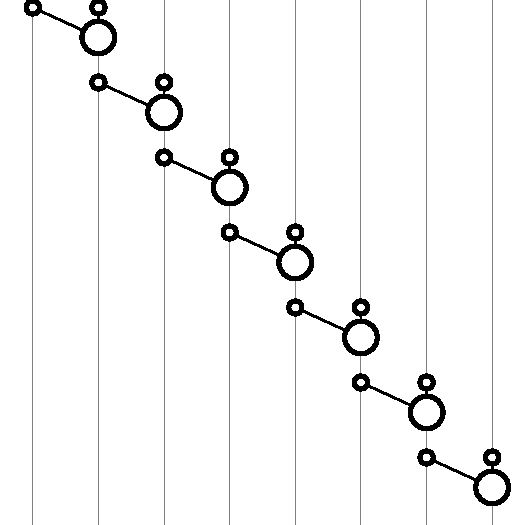
\includegraphics{serial}
  \vspace{12 pt}
  \mint{julia}|render(prefix8!(AccessArray(8),+))|
  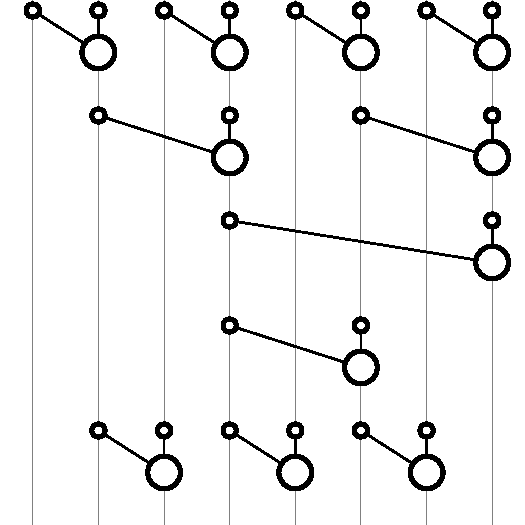
\includegraphics{tree}
  \caption{Above: operation order for the left-associative algorithm
	  \code{prefix\allowbreak\_serial!}.
	  Below: operation order for the tree algorithm \code{prefix8!}.
	  The code listing for the \code{render} function is given in
	  Section~\ref{sec:render}. This figure was rendered in Compose, a
	  Julia package for declarative vector graphics~\cite{Compose.jl}.}
   \label{fig:gates}
\end{figure}

To conclude our exposition of the scan problem, we present the \code{prefix!}
function that solves the general case of $n$ data points. While the indices are
somewhat less clear than when explicitly written out in \code{prefix8!}, the
\code{prefix!} function nonetheless preserves the double tree structure.

\begin{minted}{julia}
function prefix!(y, +)
    l=length(y)
    k=iceil(log2(l))
    #The "reduce" tree
    for j=1:k, i=2^j:2^j:min(l, 2^k)
        y[i] = y[i-2^(j-1)] + y[i]
    end
    #The "broadcast" tree
    for j=(k-1):-1:1, i=3*2^(j-1):2^j:min(l, 2^k)
        y[i] = y[i-2^(j-1)] + y[i]
    end
    y
end
\end{minted}

Again, at this point we have only written serial code that introduces more
computations than the naive algorithm \code{prefix\allowbreak\_serial!}. However, we will
argue in Section~\ref{sec:parallel-prefix} that the exact same code in
\code{prefix!} can be reused for parallel execution which can achieve speedup
over \code{prefix\allowbreak\_serial!}.

\section{Distributed computing using prefix reduction}

In this section we show how the prefix algorithm we wrote above can be run in a
distributed setting without modification. The key is to make use of overloading
using the multimethod dispatch feature of Julia.

Julia provides native support for multiprocess distributed computing based on
one-sided message passing. The basic functionality is provided by the
\code{remotecall} function, which initiates a nonblocking remote function call
and returns an explicit future (a remote pointer of type \code{RemoteRef})
whose value is retrieved by the \code{fetch} function, which is a blocking
operation. Julia also provides more convenient syntax for \code{remotecall}
with the \code{@spawn} and \code{@spawnat} macros, which automatically rewrite
Julia expressions into \code{remotecall} function calls.

We can use Julia's multiple dispatch feature to define associative operators
which act on remote data rather than local data. Julia's generic function
system allows new methods which act on remote data to be defined for functions
like \code{+} and \code{*}, which are simply functions for which the parser
supports infix notation. In effect, we can overload addition and multiplication
(or in general any binary associative function) transparently to work on remote
data.

For example, we can run the following code:

\begin{minted}{julia}
#Start a Julia process on every available core
#addprocs(n) adds n processors
#Sys.CPU_CORES is the total number of available
#CPU cores
#nprocs() returns the total number of Julia
#processes attached to the current master
#(including itself)
addprocs(max(0, Sys.CPU_CORES-nprocs()))

import Base.* #Extend existing generic function

#Define elementary operations on remote data
*(r1::RemoteRef,r2::RemoteRef)=
    @spawnat r2.where fetch(r1)*fetch(r2)
\end{minted}
%
This one method definition defines multiplication on remote data by
\code{fetch}ing the remote data from the process containing the data of
\code{r1}, copying the data of \code{fetch(r1)} to the memory space of the
process with id \code{r2.where}, which already stores the data of \code{r2}.
The process \code{r2.where} now contains local copies of both operands.
Assuming that the local data are of type \code{T}, the Julia code
then invokes another round of method dispatch based on the method signature
\code{*(::T, ::T)}. In this way, any data type \code{T} that supports
multiplication will now also support remote multiplication, regardless of
whether the data are scalar numbers, $N\times N$ matrices, or something else
entirely.

The main point of this paper is that the very same function \code{prefix!}
which was executed in serial in previous sections will now run in parallel,
simply by passing to it an associative operator over remote data rather than
local data. Julia's multimethods and multiple dispatch semantics allow
operations on remote data to share the same syntax as their corresponding
operations on local data, thus removing any syntactic difference between remote
and local operations. The new method for \code{*} defines new behavior
specific to \code{RemoteRef}s, which are Julia's explicit futures. With this
new method defined in the current scope, running \code{prefix!(y, *)} will
automatically compute cumulative products on remote data if \code{y} is an
array of \code{RemoteRef}s. Julia will automatically dispatch on the
\code{*(r1::RemoteRef, r2::RemoteRef)} method within the inner loops of
\code{prefix!} by comparing the types of the data elements of \code{y} with
method signatures defined for \code{*}.

\subsection{Parallel prefix}
\label{sec:parallel-prefix}

We now run the \code{prefix!} function in parallel. The remote operations
\code{*(r1::RemoteRef, r2::RemoteRef)} contain blocking operations implied by
\code{fetch(r1)}, and Julia dynamically schedules all remote operations
simultaneously so long as they are not waiting on the result of a \code{fetch}
operation. The scheduling and dependency structure of \code{prefix!} thus
results in all operations in each stage of the tree being executed
simultaneously. Neglecting overhead from communication latency and bandwidth,
the total execution time of \code{prefix!} depends only on the depth of the
trees defined by the inner loops of \code{prefix!} and visualized in
Figure~\ref{fig:gates}.

From the indices of each loop in \code{prefix!} for $l$ data points, the first
tree has at least one operation at depth $k$ for $l \ge 2^k$, and therefore the
depth of the entire tree is $k = \floor{\log_2 l}$. Similarly, the second tree
has at least one operation at depth $k$ for $l \ge 3\cdot2^{k-1}$, and hence
has depth $k = 1 + \floor{log_2 \frac l 3}$. Adding these depths and assuming
that we distribute one datum per processor, we therefore obtain the theoretical
speedup ratio for $p$ processors running \code{prefix!} over
\code{prefix\allowbreak\_serial!} as:

\begin{equation}
    r (p) = \frac {p-1} {\floor{\log_2 p} + 1 + \floor{\log_2 \frac p 3}}.
    \label{eq:scaling-theory}
\end{equation}

Figure~\ref{fig:scaling} summarizes benchmark timings for a sample problem
where we generated $p$ square random matrices with Gaussian entries of size $n
= 4096$ and timed how long it took to multiply these matrices together.  We
specifically left out the time needed to broadcast the data to the remote
processes, so as to focus only on the execution times of the kernels of
interest. We also took care to disable the garbage collector. Julia, like many
high-level dynamic languages, provides a garbage collector to aid in memory
management. Julia v0.3.1 uses a simple stop-the-world, non-moving, precise mark
and sweep garbage collector, where deallocation and finalization of garbage
objects may not happen immediately after objects become unused\footnote{The
code for Julia's garbage collector may be found at
\url{https://github.com/JuliaLang/julia/blob/275afc8b74b9c6ea5d34aefb8085525ff5dfc239/src/gc.c}}~\cite{McCarthy1960}.
Therefore, it becomes important to factor out the possible effects of
stop-the-world garbage collection. We explicitly disabled garbage collection
with \code{gc\_disable()} before running each kernel, then re-enabled garbage
collection with \code{gc\_enable()} after running each kernel. As an additional
precaution, we timed the kernels multiple times and took the minimum time for
each kernel so as to reduce fluctuations due to general nondeterministic
delays.

\begin{figure}
  \centering
  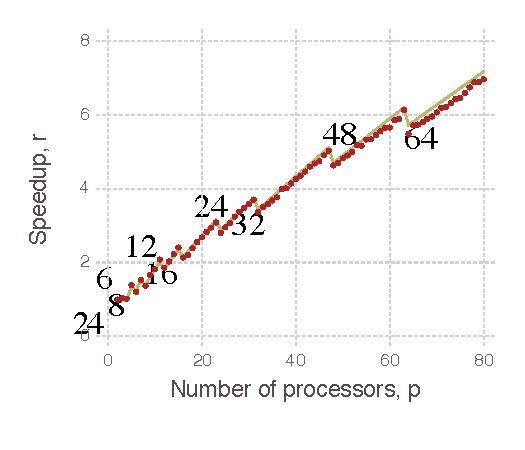
\includegraphics{scaling}
  \caption{Weak scaling of the prefix sum kernels. Speedup ratios are the
  timings for \code{prefix!} over \code{prefix\allowbreak\_serial!}. Plotted as
  a solid line is the theoretical speedup ratio $r(p)$ of
  Equation~\ref{eq:scaling-theory}. This figure was rendered in Gadfly, a
  Julia package for native plotting and visualization~\cite{Gadfly.jl}.}
  \label{fig:scaling}
\end{figure}

The empirical timings shown in Figure~\ref{fig:scaling} show excellent
agreement with the theoretical prediction of Equation~\ref{eq:scaling-theory},
with slight deterioration for $p>40$ cores reflecting the increased
communication overhead. The steps in the graph are as predicted by theory,
arising from the depth of the computation tree growing by one to accommodate
the extra data.

\section{Polymorphism for dynamic code visualization}

Earlier, we showed in Figure~\ref{fig:gates} visualizations demonstrating the
double tree structure of the Brent--Kung parallel prefix algorithm and also the
cascading or rippling structure of the serial scan. These figures were
generated programmatically from the exact same kernels \code{prefix!} and
\code{prefix\_serial!} used to perform the computations.

Many visualizations of algorithms are bespoke; the visual representation of the
algorithm is completely decoupled from implementations in executable code.
Alternatively, one may envision generating visualizations of algorithms
directly from code implementations. Visualizations of algorithms can be
generated by static analysis: feed the compute kernel into another program as
data to compute the internal data flow. The static approach, however, is
tantamount to reimplementing the compiler to generate the correct execution
trace, from which the data flow can be inferred. Instead, one can employ
dynamic analysis, instrumenting the program much like a debugger. Conventional
debuggers either work on modified code with explicit instrumentation hooks
embedded into the original kernel, or run the program in a special virtual
machine with instrumentation hooks built into the low-level machine
architecture. In these dynamic analyses, the execution trace is reconstructed
from the global machine state, and again the data flow is inferred from the
execution flow.

In this section, we describe a simple way to generate visualizations
programmatically by instrumenting the interface of specific data object, namely
arrays. Instrumentation at this level retains the advantage of composing with
unmodified compute kernels, but does not require the sophisticated
infrastructure of an instrumented virtual machine, and reuses the static
analysis of the original compiler. Furthermore, the instrumentation occurs at
the level of individual variables, enabling highly selective traces
which are cheaper than conventional approaches which instrument the entire
program state. Additionally, the instrumentation measures the data flow
directly, rather than inferring it from global execution flow. The resulting
visualization provides an individual variable's point of view of what happens
over the course of a computation.

Our implementation in Julia takes advantage of genericity in the object model.
Unlike most traditional object-oriented paradigms, which focus on data
encapsulation~\cite{Cardelli1985}, the object model in Julia focuses on the
interface to objects provided by method calls~\cite{Mitchell1988}. Making the
behavior primary over the data contents lends more naturally to data
abstraction~\cite{Mitchell1988,Abadi1996}, and furthermore admits less conventional
object models involving multimethods and multiple dispatch~\cite{Castagna1997}.

\code{Array}s in Julia are containers of a given size (possibly with multiple
dimensions) and element type. The basic array interface for Julia provides size
and indexing semantics~\cite{Bezanson2014}. The basic interface is provided by
three functions:

\begin{description}
	\item[\code{length(A)}] returns the number of elements in the array
	      \code{A},
      	\item[\code{getindex(A, idx...)}] retrieves the element of the array
	      \code{A} with index \code{idx},
      	\item[\code{setindex!(A, val, idx...)}] puts the value \code{val} in
	      the array \code{A} at the index \code{idx}.
\end{description}

The Julia parser also provides syntax sugar for the latter two operations: code
like

\mint{julia}|A[i] = A[j] + A[k]|
%
is desugared into code of the form

\begin{minted}{julia}
x = getindex(A, j)
y = getindex(A, k)
z = x + y
setindex!(A, z, i)
\end{minted}

\TODO{Rewrite the next two paragraphs}

The nice thing is you can write a custom type that implements \code{getindex} and \code{setindex!}. You don't have to go crazy and implement ALL the indexing semantics of Julia arrays, just the methods that are relevant to your specific application. In this problem all that is really needed is the indexing semantics of a single element.

Now all we have to do is to introduce a custom type that doesn't really do anything but instead records every \code{getindex} and \code{setindex!} operation performed on it. To satisfy the minimum requirements of the prefix reduction algorithm all we need at the moment is for \code{getindex} to return \code{nothing} and to define a dummy method for the associative operator \code{+} that operates on \code{nothing}. \code{nothing} is a value of the special singleton type \code{Void}, akin to Python's \code{none} or Haskell's \code{Nothing}.

Here is a code listing of implementing the trace type

\begin{minted}{julia}
import Base: getindex, setindex!, length

type AccessArray
    length :: Int
    read :: Vector
    history :: Vector
    AccessArray(length)=new(length, {}, {})
end

length(A::AccessArray)=A.length

function getindex(A::AccessArray, i)
    push!(A.read, i)
    nothing
end

function setindex!(A::AccessArray, x, i)
    push!(A.history, (A.read, {i}))
    A.read = {}
end

#Dummy operator
+(a::Void, b::Void) = nothing
\end{minted}

\TODO{Elaborate}

\section{Proving correctness}

In Section~\ref{sec:prefix} we introduced several different kernels to compute
scans. But how do we know that these kernels compute the prefix sum correctly?
Each of these kernels have exactly the same function signature \code{(y,
+)} representing the data \code{y} and associative binary operator \code{+}.
It turns out that the inputs \code{(y, +)} to the scan algorithm turn out to
have exactly the algebraic structure of a monoid, if the domain of array
elements \code{y[i]} contains an identity under the operation \code{+}. The
monoidal structure has been used in at least two ways to prove correctness.
First, \cite{Hinze2004} constructed a formal algebra that allows correctness of
circuits to be proved by derivation: all circuits which are equivalent to a
known correct circuit, up to certain algebraic transformations, will all be
correct. However, the algebraic proof of correctness is not constructive and
does not lend itself easily to programmatic verification. Second and more
recently, \cite{Chong2014} proved that the correctness of a kernel can be
demonstrated by proving correctness for the interval monoid
(Definition~\ref{def:intervalmonoid}), which formalizes the notion of indexing
the subarrays being accessed over the course of the prefix sum computation. The
latter method of proof is easy to verify programmatically.

In this section, we show how polymorphism allows the same Julia code written in
previous sections for practical computations to also be used in the formal
setting of verifying correctness. For convenience, we quote the definition of
the interval monoid:

\begin{definition}{\cite[Definition 4.3]{Chong2014}}
\label{def:intervalmonoid}
	
The \textit{interval monoid} $I$ has the elements

\begin{equation}
	\mathbb S_I = \left\{ (i_1, i_2) \in \mathrm{Int} \times \mathrm{Int} \;\vert\; i_1 \le i_2  \right\} \cup \{\mathbf 1_I, \top \}
\end{equation}
%
and a binary operator $\oplus_I$ defined by:

\begin{subequations}
\begin{align}
	\mathbf 1_I \oplus_I x = x \oplus_I \mathbf 1_I &= x \textrm{ for all } x \in \mathbb S_I \\
	\top \oplus_I x = x \oplus_I \top &= \top \textrm{ for all } x \in \mathbb S_I \\
	(i_1, i_2) \oplus_I (i_3, i_4) &= \begin{cases} (i_1, i_4) &\textrm{if } i_2 + 1 = i_3 \\
		\top &\textrm{otherwise.}
\end{cases}
\label{eq:intervalplus}
\end{align}
\end{subequations}

\end{definition}

The elements $(i, j) \in \mathbb S_I$ are abstractions of array indexing
operations which produce array slices; they are produced by Julia code like
\code{y[i:j]} where \code{i:j} is of type \code{UnitRange} and is a range of
unit stride representing the set $\{i, i+1, \dots, j\}$. The definition of
$\oplus_I$ in \eqref{eq:intervalplus} formalizes the notion of combining the
results from the subarrays \code{y[i:j]} and \code{y[j+1:k]} to get the result
for the subarray \code{y[i:k]}.  The identity element $\mathbf 1_I$ formalizes
an empty interval, while the annihilator $\top$ encodes noncontiguous ranges,
which correspond to partial sums which cannot be represented by slicing with a
\code{UnitRange}.

The key insight of \cite{Chong2014} is that correct computations of prefix sums
cannot generate noncontiguous elements $\top$, otherwise they would by
definition violate the prefixing property \code{prefix!(y[1:j+1], +) =
prefix!(y[1:j], +) + y[j+1]}.\\
From this insight, the authors of \cite{Chong2014} derive two correctness
results:

\begin{enumerate}
		
\item 	A function that computes the prefix sum in serial is correct for $n$
	data points if and only if that function computes the correct answer
	for the input \\
	$\left(\left((1, 1), (2, 2), \dots, (n, n)\right),
	\oplus_I\right)$\footnote{Our presentation differs from the original
	only in that Julia arrays are 1-based, in contrast to C/OpenCL arrays
	studied in the original~\cite{Chong2014}, which are 0-based.}
	~\cite[Theorem 4.5]{Chong2014}.
	Furthermore, the correct answer is $\left((1, 1), (1, 2), \dots, (1, n)
	\right)$, as the $k$th partial sum involves summing the subarray
	\code{y[1:k]}.
	
\item	A function that computes the prefix sum in parallel is correct if it is
	free of data races and its equivalent serialization is
	correct~\cite[Theorem 5.3]{Chong2014}.

\end{enumerate}

We can use these results directly to verify the correctness of the Julia code
we have written in earlier sections. By construction, the \code{fetch}es on
\code{RemoteRefs} insert implicit synchronization barriers and thus the
parallel code is free of data races. Thus only the serial correctness result
needs to be verified explicitly.

Julia allows us to encode the interval monoid directly from the definition. A
convenient feature of Julia is the ability to use abstract data types as
singleton values: Julia types are values, and types can be used as singleton
values using the \code{Type\{T\}} construct. Thus, the domain $\mathbb S_I$ can
be written as a Julia type \code{S}, which is the \code{Union} (type union) of:

\begin{itemize}
	\item \code{UnitRange},
	\item \code{Type\{Id\}}, the identity singleton $\mathbf 1_I$, and
	\item \code{Type\{Tee\}}, the annihilator singleton $\top$.
\end{itemize}

With this mapping of the abstract interval monoid domain $\mathbb S_I$ onto
Julia types, Definition~\ref{def:intervalmonoid} translates directly into the
following code:

\begin{minted}[mathescape,texcl]{julia}
#S is the interval monoid $\mathbb{S}_I$ of Definition \ref{def:intervalmonoid}
abstract Tee #$\top$
abstract Id  #$\mathbf{1}_I$
typealias S Union(UnitRange, Type{Tee}, Type{Id})

#$\oplus_I$
+(I::UnitRange, J::UnitRange) = #$+_1$ 
    I.stop+1==J.start ? (I.start:J.stop) : Tee
+(::Type{Id}, ::Type{Id}) = Id  #$+_2$
+(I::S, ::Type{Id}) = I         #$+_3$
+(::Type{Id}, I::S) = I         #$+_4$
+(I::S, J::S) = Tee             #$+_5$
\end{minted}

The Julia method dispatcher chooses the most specific method that matches the
type signature of a given set of arguments~\cite{Bezanson2012}. Thus even
though \code{+} may appear to be ambiguously defined for inputs with the type
signature \code{(::Unit\-Range, ::UnitRange)}, which matches both $+_1$ and $+_5$
methods, Julia resolves the ambiguity in favor of $+_1$ which has the more
specific type signature, since by definition \code{UnitRange} is a subtype of
\code{S}. However, the method $+_2$ is necessary to resolve the ambiguity
between $+_3$ and $+_4$: Julia uses symmetric multiple dispatch, so that the
positions of the arguments are not used to resolve
ambiguities~\cite{Bezanson2012}. As a result, inputs with type signature
\code{(::Type\{Id\}, ::Type\{Id\})}, which lie in the intersection of the type
signatures of $+_3$ and $+_4$, have to be special-cased. Bearing these rules in
mind, it is straightforward to verify that the definition of \code{+} in the
code block above is equivalent to that of $\oplus_I$ in
Definition~\ref{def:intervalmonoid}. Julia's method dispatch rules allow
\code{+} to be defined in a way that reveals the catch-all nature of $\top$:
method $+_5$, which returns \code{Tee}, is dispatched only when none of the
other methods matches the type signature of the given arguments.
Figure~\ref{fig:dispatch} summarizes the method dispatch table.

\begin{figure}
  \centering

  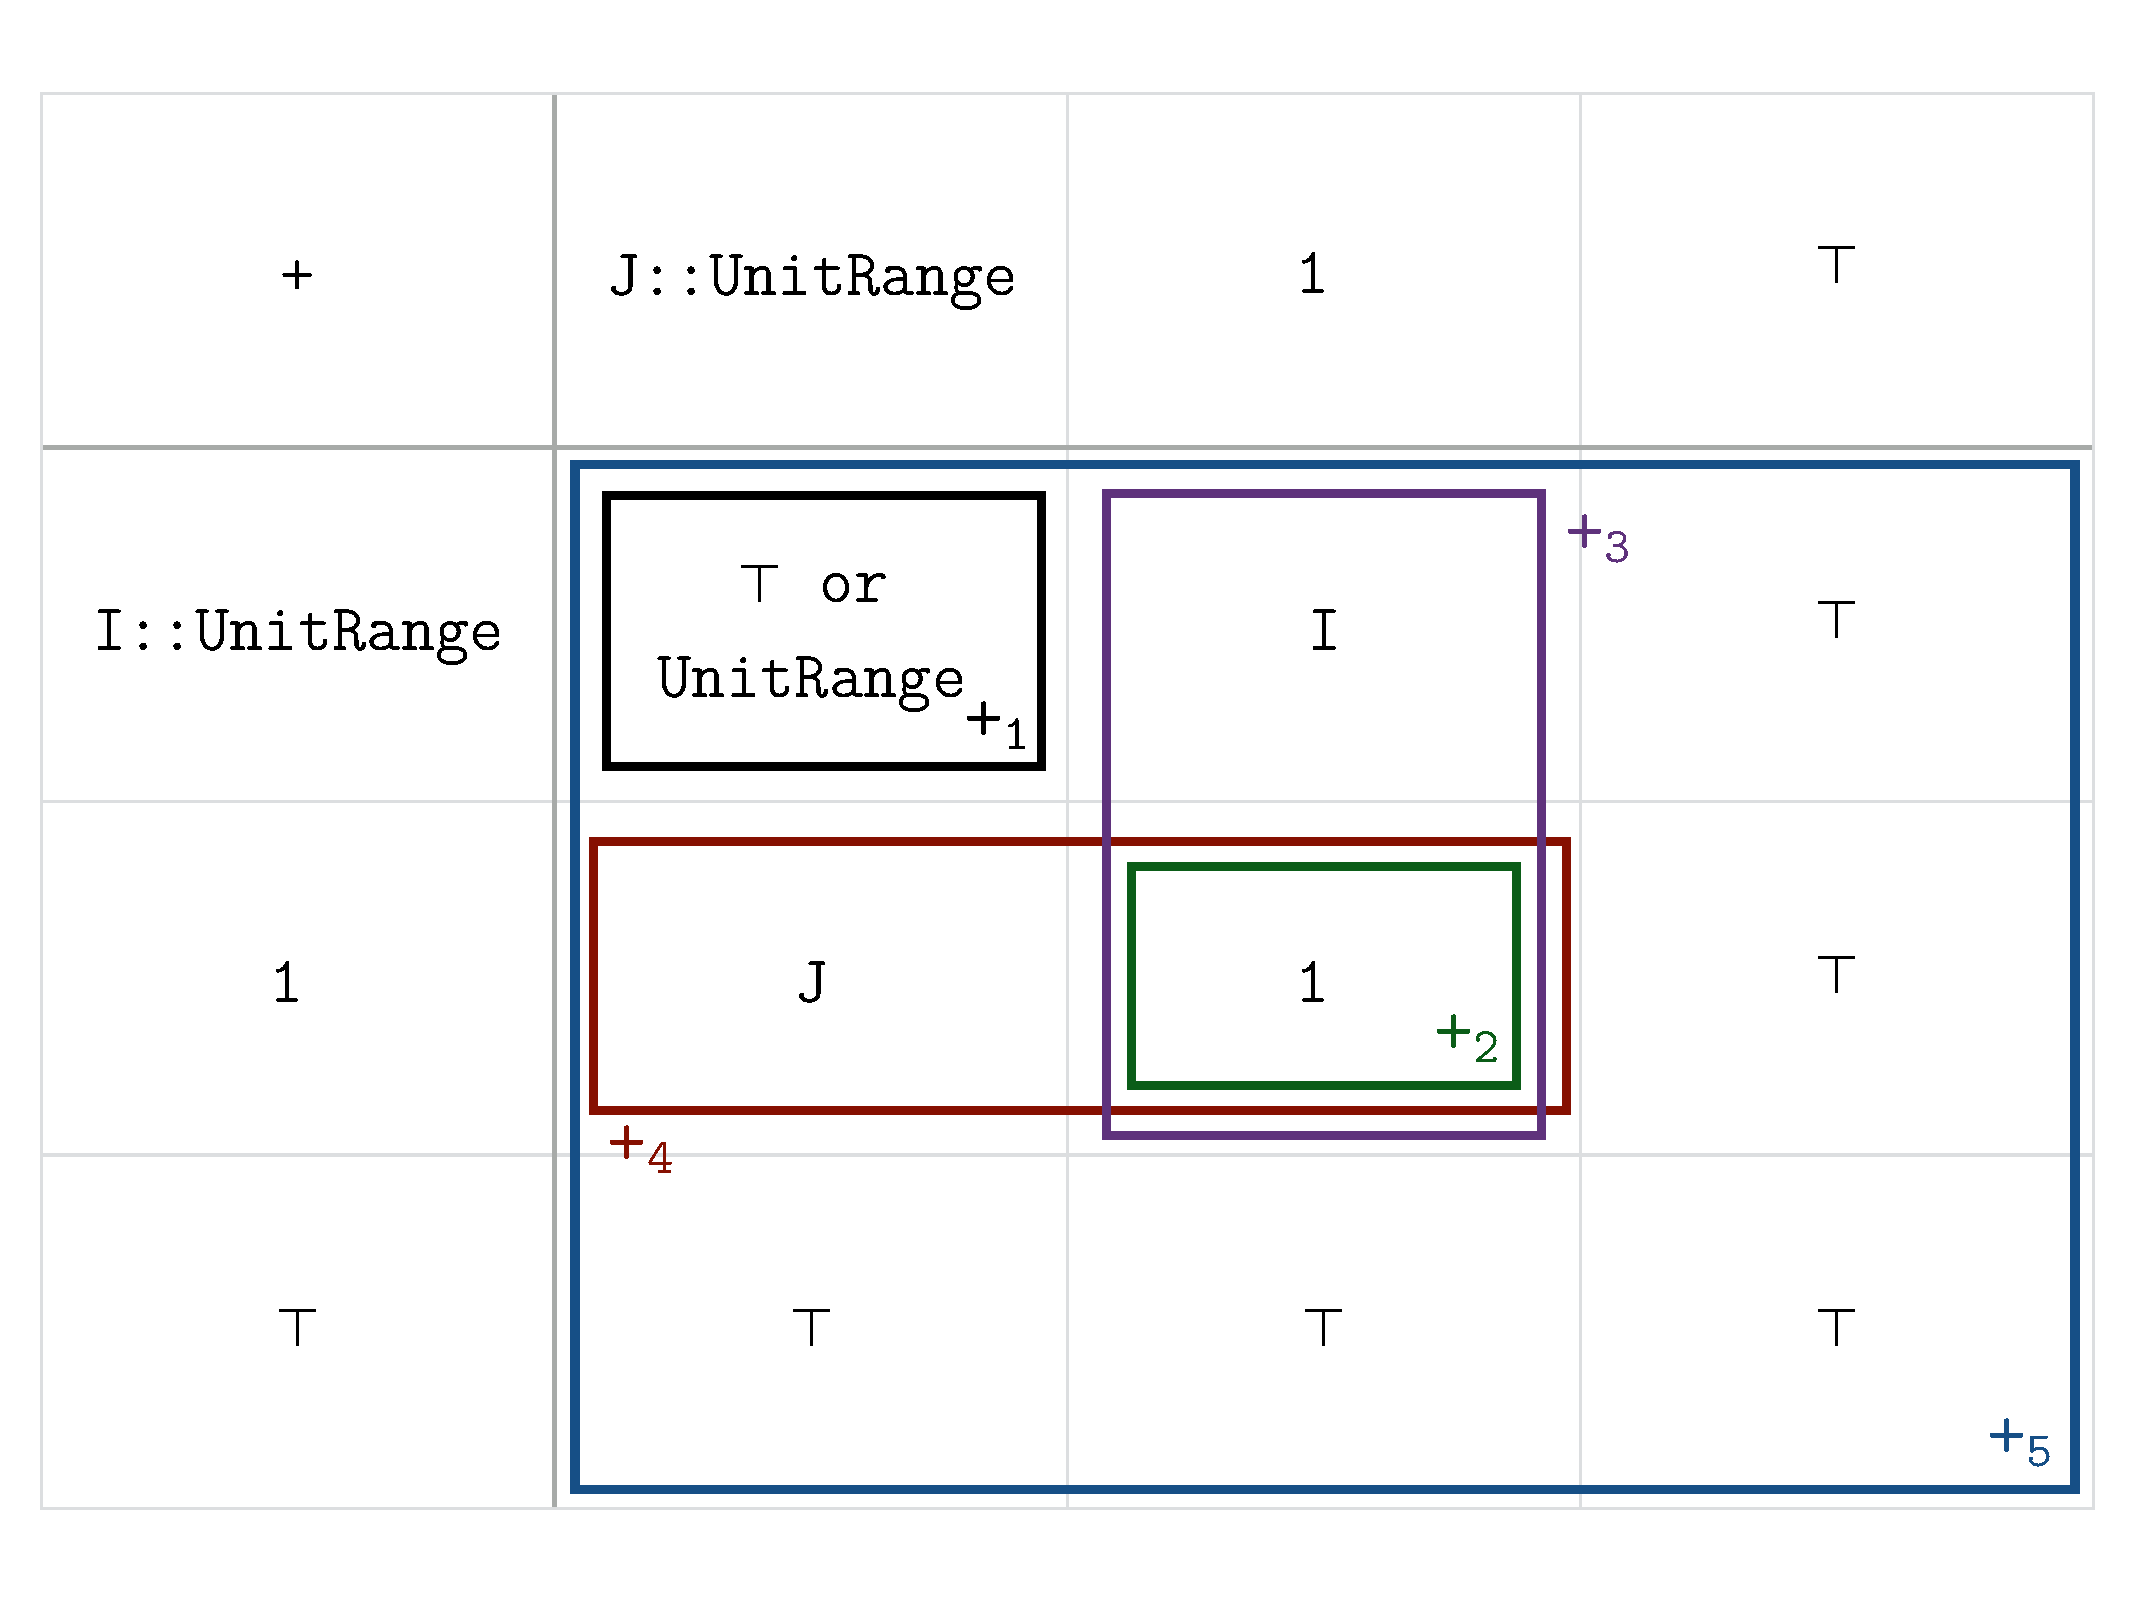
\includegraphics[width=.9\columnwidth]{intervaldispatch}
  \caption{Dispatch table for the monoid operator $\oplus_I$.}
   \label{fig:dispatch}
\end{figure}

Verifying some function \code{kernel} for the problem size \code{n} simply
reduces to writing the assertion:

\begin{minted}{julia}
#Test that kernel is correct for problem size n
@assert kernel([k:k for k=1:n],+)==[1:k for k=1:n]
\end{minted}

Attempting to verify an incorrect kernel results in at least one $\top$ being
produced during the computation, thus poisoning the program state and
precipitating type conversion errors of the form

\begin{minted}{jlcon}
`convert` has no method matching
convert(::Type{UnitRange}, ::Type{Tee})
\end{minted}
%
which arise from the inability of noncontiguous ranges to be expressed as
\code{UnitRange}s.

Julia thus allows for the same kernels used for computation to be verified
directly without any rewriting or translation, simply by exploiting the
polymorphism arising from the generic nature of prefix sum kernels, and
composing such generic functions with appropriate choices of input data types
and associative operators over those types.

\TODO{Two-language problem for formal verification?}

\section{Related work}

\TODO{Cleanup}

Julia lets us encode the interval monoid very naturally, unlike the original work where they had to encode the monoid in C++/OpenCL types~\cite{Chong2014}.

What do other languages do?

Other languages also provide scan primitives like APL~\cite{Iverson1962,Iverson1979}, ZPL~\cite{Chamberlain2000}.

MPI provides the \code{MPI\_scan} primitive~\cite{Snir1995,MPI}, and in MPI-2, also the \code{MPI\_Exscan} primitive for exclusive scan.~\cite{MPI2}

Other approaches wish they have genericity, like the Thrust C++ library which uses crazy C++ functors~\cite{Bell2012}.

Does Haskell have something using monoids?

Haskell Accelerate for GPU programming~\cite{Chakravarty2011}. Is it generic? Yes because it works at the code generation level, taking in expressions and emitting longer expressions that compute the prefix sum. In Haskell land these things are criticised for being not statically typed...?

In Julia we use duck typing.

Our approach is rather naive and does not account for the complexities in real world implementations, for example possible synchronicity issues produced by higher levels of the broadcast and reduce trees that could result in bus saturation. In principle this can be handled at the scheduler level in the system but we currently don't have the capabilities to do so in Julia.

\section{Conclusions and outlook}

\TODO{Cleanup}

We used polymorphism in many different ways. For a single set of kernels, we used them to do real computations on numbers and matrices, and also on \code{AccessArray}s to trace through the code to do some visualization, and also on the interval monoid $(\mathbb S_I, \oplus_I)$ to verify program correctness.

Here is a way to visualize parallel algorithms and study their correctness. First we show that with pure operator polymorphism we can explicitly show the equivalence of a parallel algorithm and a sequential execution that accomplishes the same computations. This can be used to prove the correctness of a parallel algorithm.

Other variants: e.g. Snir~\cite{Kruskal1985}, Koc~\cite{Egecioglu1992}, doubly pipelined~\cite{Sanders2006}, harmonically scheduled~\cite{Wang1996}, segmented scan~\cite{Sengupta2007}.

Generalization to nonassocative binary operations~\cite{Chen1992}

Visualization is a byproduct of a correct algorithm. This is a powerful new way to understand how algorithms work.

How about something about fast multipole and variants?

\section{Acknowledgments}
We gratefully acknowledge the Julia community, especially Jake Bolewski, for insightful discussions.

Also funding.

\bibliographystyle{abbrv}
\bibliography{prefix}

\appendix

\section{The \code{render} function}
\label{sec:render}

Here are the \code{gate} type and \code{render} function used to generate the figures in Figure~\ref{fig:gates}.

\TODO{Explain assumptions in the rendering}

\begin{minted}{julia}
using Compose

type gate
    ins :: Vector
    outs:: Vector
end

function render(G::gate, x, y, y0; ri=0.1, ro=0.25)
    ipoints = [(i, y0+ri) for i in G.ins]
    opoints = [(i, y0+0.5) for i in G.outs]
    igates  = [circle(i..., ri) for i in ipoints]
    ogates  = [circle(i..., ro) for i in opoints]
    lines = [line([i, j]) for i in ipoints,
                              j in opoints]

    compose(context(units=UnitBox(0.5, 0, x, y+1)),
        compose(context(), stroke("black"),
	    fill("white"), igates..., ogates...),
        compose(context(), linewidth(0.3mm),
	    stroke("black"), lines...))
end

function render(A::AccessArray)
    #Scan to find maximum depth
    olast = depth = 0
    for y in A.history
        (any(y[1] .<= olast)) && (depth += 1)
        olast = maximum(y[2])
    end
    maxdepth = depth
    
    olast = depth = 0
    C = {}
    for y in A.history
        (any(y[1] .<= olast)) && (depth += 1)
        push!(C, render(gate(y...), A.length,
	    maxdepth, depth))
        olast = maximum(y[2])
    end
    
    push!(C, compose(context(
      units=UnitBox(0.5, 0, A.length, 1)),
      [line([(i,0), (i,1)]) for i=1:A.length]...,
      linewidth(0.1mm), stroke("grey")))
    compose(context(), C...)
end
\end{minted}

\end{document}
